% vim: set spelllang=fr foldmethod=marker:
\section{Modélisation}
\label{sa:sec:modelisation}

Nous avons détaillé la solution proposée. À présent, nous allons présenter plusieurs modèles possibles permettant de représenter cette solution, et d'en évaluer les performances selon divers critères.

%===============================================================================
    \subsection{Chaînes de Markov}

        \subsubsection{Présentation et hypothèses de travail}
Nous avons modélisé notre solution sous la forme d'un processus de Markov à temps continu (CMTC, pour chaîne de Markov à temps continu).

Notre modèle représente un cluster d'un réseau de capteurs sans fil qui vérifie les hypothèses suivantes:
\begin{itemize}
    \item seul le cluster est modélisé;
    \item le cluster contient exactement un \CH, $s$ capteurs chargés d'effectuer des mesures, et $m$ nœuds jouant le rôle de \cns\footnote{$s$ pour \textit{sensing node}, $m$ pour \textit{monitoring node}.};
    \item il existe exactement un nœud compromis parmi les $s$ capteurs;
    \item le capteur $i$ ($1 \leq i \leq s$) génère du trafic selon un processus de Poisson de paramètre $\lambda_i$;
    \item le nœud compromis $c$ génère du trafic selon un processus de Poisson de paramètre $\lambda_i$ (tel que $\forall i\in[\![1;s]\!]\backslash\{c\},\; \lambda_c\gg\lambda_i$);
    \item chaque \cn effectue une détection du trafic environnant de façon périodique, selon une distribution exponentielle de paramètre $\mu$; si un trafic anormal est observé, le \cn transmet un rapport d'anomalie au \CH;
    \item la topologie du cluster correspond à un graphe connexe: chaque nœud peut atteindre directement chacun des autres nœuds du cluster.
\end{itemize}

        \subsubsection{Modélisation}
Sous les hypothèses précédentes, notre modèle peut être représenté par une CMTC multi-dimensionnelle de taille $m$.
Il est alors exprimé sous la forme d'un $m$-uplet $x\!=\!(x_1,x_2,\dots,x_m)$ de macro-états $x_k\!=\!(x_{k_1},x_{k_2},\dots,x_{k_s},x_{k_d})$.
Chaque macro-état $x_k$    garde en mémoire le nombre de paquets détectés par le \cn $k$ ($1\leq k\leq m$).
Plus exactement, chaque $x_{k_i}$ ($1\leq i\leq s$) est un compteur, initialisé à $0$, qui est incrémenté à chaque fois que le \cn $k$ détecte un paquet en provenance du capteur $i$.
$x_{k_d}$ est une variable de type booléen, initialisée à $0$, et passée à $1$ lorsque le \cn $k$ détecte un trafic anormalement élevé.
La fonction de seuil $f:s^s\rightarrow\{0;1\}$ est utilisée par les \cns pour déterminer la nature normale ou non du trafic (elle indique si un paquet a dépassé ou non le seuil des communications dites «~normales~»).
Elle prend pour argument les valeurs des $s$ compteurs $x_{k_1},x_{k_2},\dots,x_{k_s}$ d'un macro-état $x_k$ associé à un \cn $k$, et la valeur retournée est stockée dans $x_{k_d}$.

Voici un exemple d'équation de transition pour un macro-état générique $x_k$, $1\leq k\leq m$.
Le macro-état $x$, représentant l'intégralité du système, est directement obtenu en agrégeant les différents $x_k$.
Le compteur $x_{k_c}$ représente dans la suite le nombre de messages émis par le nœud compromis et captés par le \cn $k$.
L'équation est donnée en figure~\ref{sa:fig:eqtrans}

\newlength{\fboxlinelen}
\setlength{\fboxlinelen}{\linewidth}
\addtolength{\fboxlinelen}{-4\fboxsep}
\addtolength{\fboxlinelen}{-2\fboxrule}

\begin{figure}[ht]
    \fbox{
        \begin{minipage}{\fboxlinelen}
            \begin{eqnarray*}
                x_k    & \rightarrow & \mbox{Transmission d'un capteur normal} \\
                    & \rightarrow & (x_{k_1},\dots,x_{k_i}+1,\dots,x_{k_c},  \dots,x_{k_s},0) \\
                    &             & \qquad\mbox{avec la fréquence }\lambda_{i}\!\neq\!\lambda_{c} \\ \\
                    & \rightarrow & \mbox{Transmission du nœud compromis} \\
                    & \rightarrow & (x_{k_1},\dots,x_{k_i},  \dots,x_{k_c}+1,\dots,x_{k_s},0) \\
                    &             & \qquad\mbox{avec la fréquence }\lambda_{c}\\ \\
                    & \rightarrow & \mbox{Vérification; détection d'un trafic anormal}\\
                    & \rightarrow & (0,\dots,0,\dots,0,\dots,0,1) \\
                    &             & \qquad\mbox{avec la fréquence }\mu \cdot 1_{f(x_k)\geq \mathit{seuil}} \\ \\
                    & \rightarrow & \mbox{Vérification; aucun trafic anormal détecté} \\
                    & \rightarrow & (0,\dots,0,\dots,0,\dots,0,0)  \\
                    &             & \qquad\mbox{avec la fréquence }\mu \cdot 1_{f(x_k)<\mathit{seuil}}
            \end{eqnarray*}
        \end{minipage}
    }
    \caption{Équation de transition du processus de Markov à temps continu modélisant le cluster}\label{sa:fig:eqtrans}
\end{figure}

\bigskip
Formulé autrement: le \cn $k$, dans l'état $x_k$, reçoit périodiquement les messages de chaque capteur $i$ ($1\leq i\leq s, i\!\neq\!s$): ce sont des transmissions dites «~normales~», qui surviennent avec une fréquence moyenne $\lambda_i$.
Chaque message reçu laisse le \cn $k$ dans un état presque identique, à la seule différence que le compteur $x_{k_i}$ est incrémenté de $1$.
La même chose se produit avec une fréquence $\lambda_c$ pour les messages envoyés par le nœud compromis, qui provoque à chaque fois l'incrémentation du compteur $x_{k_c}$.
Enfin, la vérification du trafic enregistré par le \cn $k$ survient avec une fréquence $\mu$.
La fonction $f$ est appliquée sur l'ensemble des $x_{k_i}$, $i$ allant de $1$ à $s$.
Si l'un des capteurs a envoyé un nombre de paquets supérieur à la valeur de seuil (\cad si l'on a $f(x_k)\geq \mathit{seuil}$), le drapeau $x_{k_d}$ est levé.
Un message d'alerte est alors envoyé du \cn $k$ au \ch.
Si, en revanche, aucune anomalie n'est à rapporter, le drapeau $x_{k_i}$ est laissé à $0$, et rien n'est envoyé.
Dans les deux cas, tous les compteurs $x_{k_i}$ sont réinitialisés à $0$, afin que la prochaine vérification soit effectuée sur des données «~fraîches~» (et pour ne pas déclencher par erreur une fausse détection par cumul des nombres de paquets envoyés d'une période sur l'autre).

La probabilité de détection du nœud compromis par le \cn $k$, notée $\Delta_k$, est la suivante:
\[\Delta_k=\sum_{x_{k_1},\dots,x_{k_s}}^\infty\pi(x_{k_1},\dots,x_{k_s},x_{k_d}=1)\]
où $\pi(x_{k_1},x_{k_2},\dots,x_{k_{s}},x_{k_d})$ représente la distribution stationnaire du macro-état $x_k\!=\!(x_{k_1},x_{k_2},\dots,x_{k_{s}},x_{k_d})$.

        \subsubsection{Limites du modèle}
Représenté sous la forme d'un processus de Markov à temps continu, le modèle suppose que la période séparant deux vérifications consécutives du trafic par un \cn est une variable aléatoire qui suit une distribution exponentielle.
Il s'agit là d'une approximation grossière; en réalité, la vérification intervient à intervalles réguliers (de longueur fixe), voire même en continu.
Il est donc nécessaire de choisir d'autres systèmes que les processus de Markov pour modéliser notre solution avec plus de précision.
Nous allons nous tourner par exemple vers des processus non-markoviens, qui ne présentent pas cette contrainte.

%===============================================================================
    \subsection{Réseaux de Petri}
Une autre représentation possible de notre système passe ainsi par l'utilisation de processus stochastiques à évènements discrets (PSED, ou DESP, \textit{Discrete-Event Stochastic Processes}, ou encore \textit{Generalized Semi-Markov Processes}).
Leur avantage principal sur les processus de Markov est leur capacité à représenter des événements dont la distribution n'est pas nécessairement exponentielle.
Plus particulièrement, nous allons utiliser des réseaux de Petri stochastiques généralisés étendus.

        \subsubsection{Présentation des réseaux de Petri stochastiques généralisés étendus}
\label{sa:subsubsec:presRPSGE}
Les réseaux de Petri stochastiques généralisés (RPSG) sont une classe de réseaux de Petri destinée à modéliser des processus stochastiques.
Leur version étendue (RPSGE) permet de représenter des transitions dont les délais sont distribués de façon quelconque~\cite{ABCDF95}.
Il s'agit d'un langage de haut niveau permettant de représenter des processus stochastiques à événements discrets (PSED, ou processus semi-markoviens généralisés, PSMG), qui au contraire des processus markoviens «~classiques~» ne sont pas limités à la représentation d'événements à distribution exponentielle.
RPGSE reprend, à quelques différences près, les définitions, la syntaxe et la représentation graphique des réseaux de Petri classiques, enrichis par des propriétés supplémentaires portant sur les transitions.
Ces dernières sont dites soit \textit{immédiates}, soit \textit{minutées}.
Elles sont de plus caractérisées par les éléments suivants:
\begin{enumerate}
    \item une distribution qui détermine de façon aléatoire le délai écoulé avant que la transition ne soit franchie;
    \item une priorité qui établit de façon déterministe la transition à franchir en premier, en cas d'égalité;
    \item un poids qui est utilisé pour tirer de façon aléatoire la transition à franchir en premier, en cas de conflits sur le délai écoulé et sur les priorités.
\end{enumerate}

Nous utilisons deux types de transitions minutées:
\begin{itemize}
    \item les distributions minutées exponentiellement distribuées (marquées dans les figures qui suivent par des rectangles vides, voir par exemple la transition \textsf{T1} sur l'exemple de gauche de la figure~\ref{sa:fig:gspnex1});
    \item les distributions minutées distribuées de façon déterministe (marquées dans les figures qui suivent par des rectangles bleus, voir par exemple la transition \textsf{T1} sur l'exemple de droite de la figure~\ref{sa:fig:gspnex1}).
\end{itemize}
Les transitions immédiates sont marquées par des rectangles pleins et noirs (voir par exemple la transition \textsf{T2} dans les exemples de la figure~\ref{sa:fig:gspnex1}).
Nous avons aussi recours à des arcs inhibiteurs.
Il s'agit d'arêtes dont la flèche sur les représentations graphiques est remplacée par un cercle (par exemple, l'arc reliant la place \textsf{P1} à la transition \textsf{T2} dans l'exemple de droite de la figure~\ref{sa:fig:gspnex1}), et accompagnées d'un chiffre.
Les règles de franchissement des transitions sont légèrement différentes avec ces arcs, puisque ces franchissement ne peuvent être effectués que si le nombre de jetons en amont de la transition est strictement inférieur au nombre indiqué sur l'arc.
Par exemple, sur la partie droite de la figure~\ref{sa:fig:gspnex1}, la transition \textsf{T2} peut être franchie, car \textsf{P1} ne contient que deux jetons (on a bien $2<3$).
\begin{figure}[ht]
    \centering
    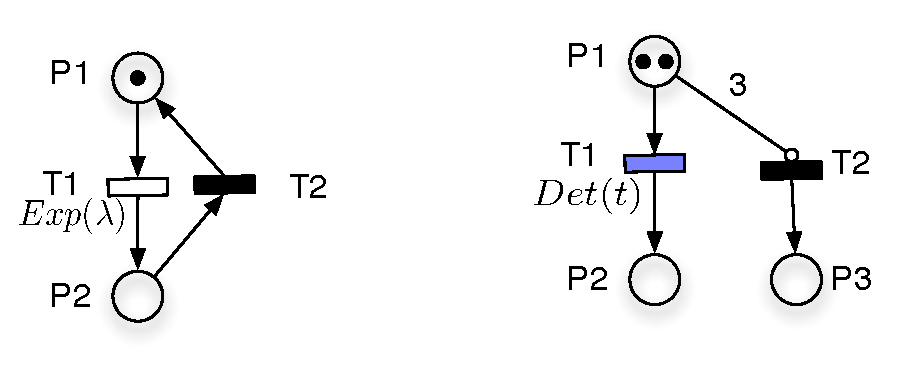
\includegraphics[width=.8\linewidth]{\chapterfig/GSPNex1.pdf}
    \caption{Exemples simples d'eGSPN: transitions immédiates, transition minutée et arcs inhibiteurs}\label{sa:fig:gspnex1}
\end{figure}

        \subsubsection{Modélisation des nœuds}
Nous allons procéder par étapes en modélisant:
\begin{enumerate}
    \item les nœuds capteurs «~simples~»;
    \item les \cns élus de manière statique;
    \item les \cns élus de manière dynamique (dont la modélisation diffère légèrement).
\end{enumerate}

            \paragraph{Modélisation des capteurs simples}
Le comportement des capteurs basiques est simple: chaque capteur $i$ envoie des paquets selon un processus de Poisson de paramètre $\lambda_i$.
Ce comportement est modélisé par le RPSG présenté en figure~\ref{sa:fig:snodegspn}.
\begin{figure}[ht]
    \centering
    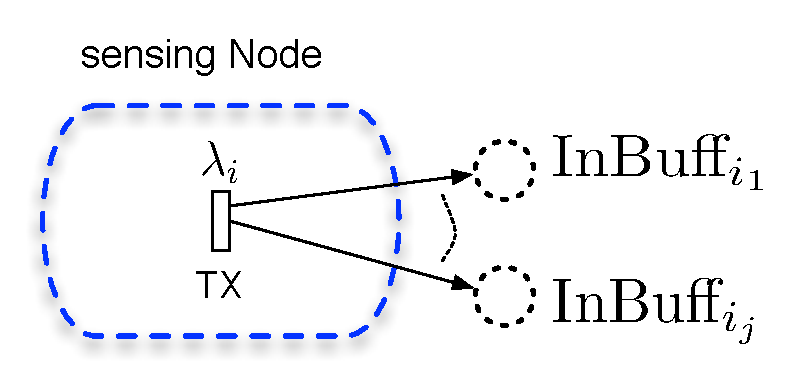
\includegraphics[width=.5\linewidth]{\chapterfig/sNode_GSPN.pdf}
    \caption{Modèle RPSG d'un nœud capteur simple}\label{sa:fig:snodegspn}
\end{figure}
Le nœud est symbolisé par les pointillés bleus.
Dans ce nœud $i$ se trouve une unique transition \textsf{TX}, sans place en entrée, autrement dit: toujours active.
Elle est minutée, avec une distribution exponentielle de paramètre $\lambda_i$: chaque événement correspond à l'envoi de jetons sur tous ses arcs sortants.
Ces arcs sont rattachés à la place \textsf{InBuff$_{i_j}$} de chacun des nœuds voisins du nœud $i$ (on trouve donc autant d'arcs sortants que de nœuds voisins).
L'intégralité de la fonction de mesure et d'envoi des données utiles du réseau de capteurs peut être modélisée par plusieurs éléments représentés par ce «~modèle de nœud~».
Un nœud compromis $c$ sera également représenté selon le même modèle, avec un paramètre $\lambda_c$ plus élevé que les autres $\lambda_i$.

            \paragraph{Modélisation des \cns élus de façon statique}
Un \cn élu de façon statique joue uniquement son rôle de \cn: il monitore le trafic, mais n'effectue pas de mesure sur son environnement.
Le modèle RPGSE associé à ce type de nœud est présenté en figure~\ref{sa:fig:cnodegspn1}.
\begin{figure}[ht]
    \centering
    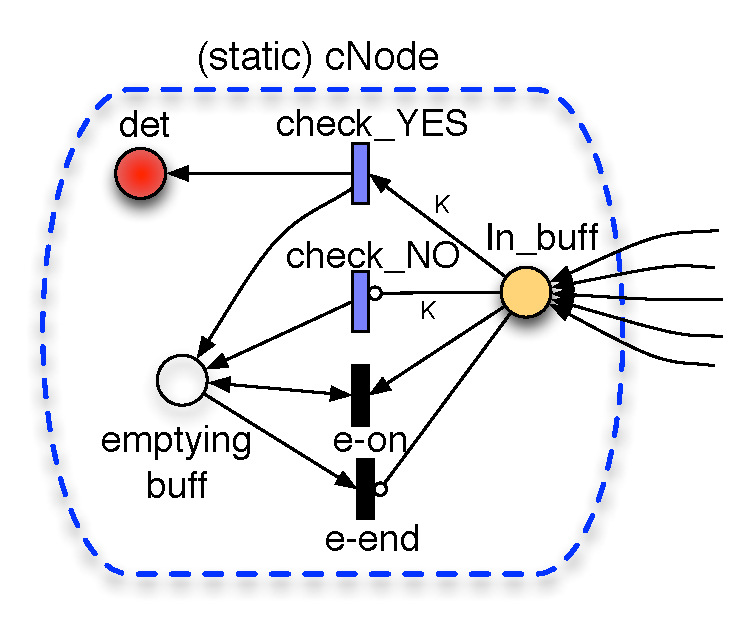
\includegraphics[width=.6\linewidth]{\chapterfig/cNode_GSPN.pdf}
    \caption{Modèle RPSGE d'un \cn élu de manière \emph{statique}}\label{sa:fig:cnodegspn1}
\end{figure}
La place \textsf{In\_buff} représente le tampon contenant les messages reçu par le nœud.
Un jeton arrivant dans cette place (depuis un nœud «~normal~») représente un message capté par le \cn\footnote{En réalité, il devrait y avoir une place \textsf{In\_buff$_i$} distincte pour les jetons provenant de chaque nœud voisin $i$ du \cn. Pour simplifier la représentation, tous les jetons arrivant au modèle du nœud sont rassemblés dans une place unique.}.
La vérification du respect de la valeur seuil $K$ pour le trafic est réalisée à intervalles de temps constants.
Les transitions \textsf{check\_YES} et \textsf{check\_NO} sont «~activées~» au bout de chaque période, et servent à assurer la vérification.
S'il y a au moins $K$ jetons dans la place, la transition \textsf{check\_YES} est franchie.
Un jeton est alors placé dans la place \textsf{det}, et fait en quelque sorte office de drapeau levé pour indiquer la détection d'un trafic anormal.
L'arrivée d'un jeton dans la place \textsf{det} déclenche l'envoi d'un message d'alerte au \ch.
Si, en revanche, il y a moins de $K$ jetons dans la place \textsf{In\_buff}, aucun jeton n'est produit dans la place \textsf{det}.
Dans un cas comme dans l'autre, la place \textsf{emptying~buff} reçoit un jeton (soit par \textsf{check\_YES}, soit pat \textsf{check\_NO}).
Un jeton dans cette place permet de vider le tampon \textsf{In\_buff}: la transition \textsf{e-on} consomme le jeton de la place \textsf{emptying~buff}, et un jeton de \textsf{In\_buff}.
Un nouveau jeton est créé dans \textsf{emptying~buff}.
Le processus est répété jusqu'à ce que la place \textsf{In\_buff} soit vide; dans ce cas, la transition \textsf{e-end} est franchie et ne produit rien, mais met fin à la consommation des jetons.
Les étapes permettant de vider le tampon ne consomment pas de temps, et permettent de repartir avec un compteur neutre pour la période qui mènera à la vérifiation suivante.

            \paragraph{Modélisation des \cns élus de façon statique}
Le modèle RPGSE représentant le \cn élu de façon dynamique ressemble à son homologue élu de façon statique.
Cependant, en raison de l'élection dynamique, tous les nœuds vont assumer périodiquement le rôle de \cn et le rôle de capteur simple.
Il est donc nécessaire d'ajouter, aux places et transitions des précédents \cns, une place \textsf{cNode} ainsi qu'une transition toujours autorisée, associée à une distribution exponentielle.
La première permet d'indiquer à chaque instant si le nœud joue le rôle de \cn (si la place contient un jeton) ou bien de capteur simple (cas contraire).
La seconde permet de produire des jetons selon un processus de Poisson lorsque le nœud fait office de capteur simple (dans ce cas la place \textsf{cNode} est vide et l'arc inhibiteur autorise le franchissement de la transition \textsf{TX}; le nœud se comporte exactement comme avec le modèle de la figure~\ref{sa:fig:snodegspn}).
Le modèle est représenté sur la figure~\ref{sa:fig:cnodegspn2}.
\begin{figure}[ht]
    \centering
    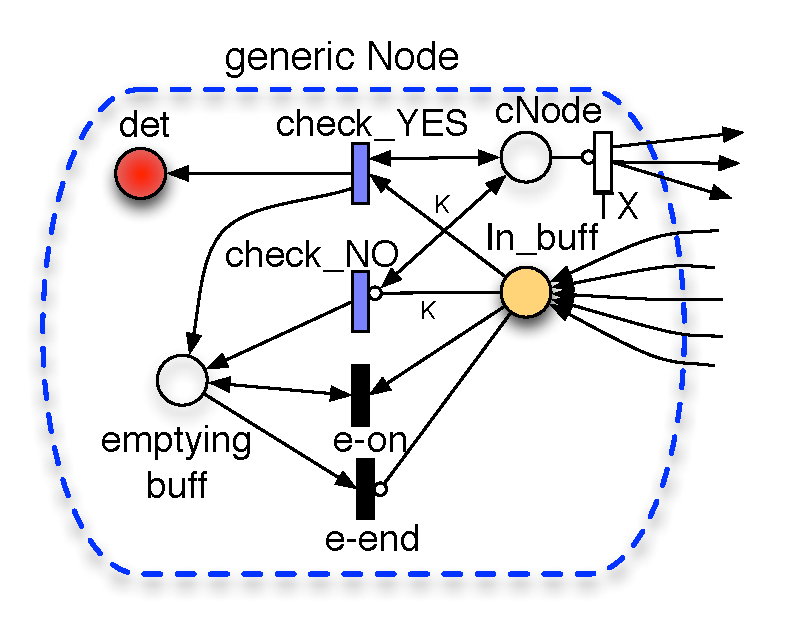
\includegraphics[width=.6\linewidth]{\chapterfig/genNode_GSPN.pdf}
    \caption{Modèle RPSGE d'un \cn élu de manière \emph{dynamique}}\label{sa:fig:cnodegspn2}
\end{figure}

        \subsubsection{Modélisation du cluster}

            \paragraph{\cns élus de façon statique}
Maintenant que la représentation des nœuds individuels a été donnée, nous sommes en mesure de modéliser notre réseau.
Nous travaillons toujours dans un unique cluster.
Pour simplifier la représentation graphique, nous choisissons de représenter un cluster comportant un total de neuf nœuds placés sur une grille de dimensions $3\times3$.
Parmi ces nœuds, deux exactement jouent le rôle de \cn (les nœuds \textsf{3} et \textsf{4} dans notre cas), et un exactement (le nœud \textsf{1}) est un capteur compromis (distinct des \cns).
Cette représentation peut être facilement étendue pour modéliser le réseau tout entier.
La représentation du cluster est donnée en figure~\ref{sa:fig:petricluster}.
\begin{figure}[ht]
    \centering
    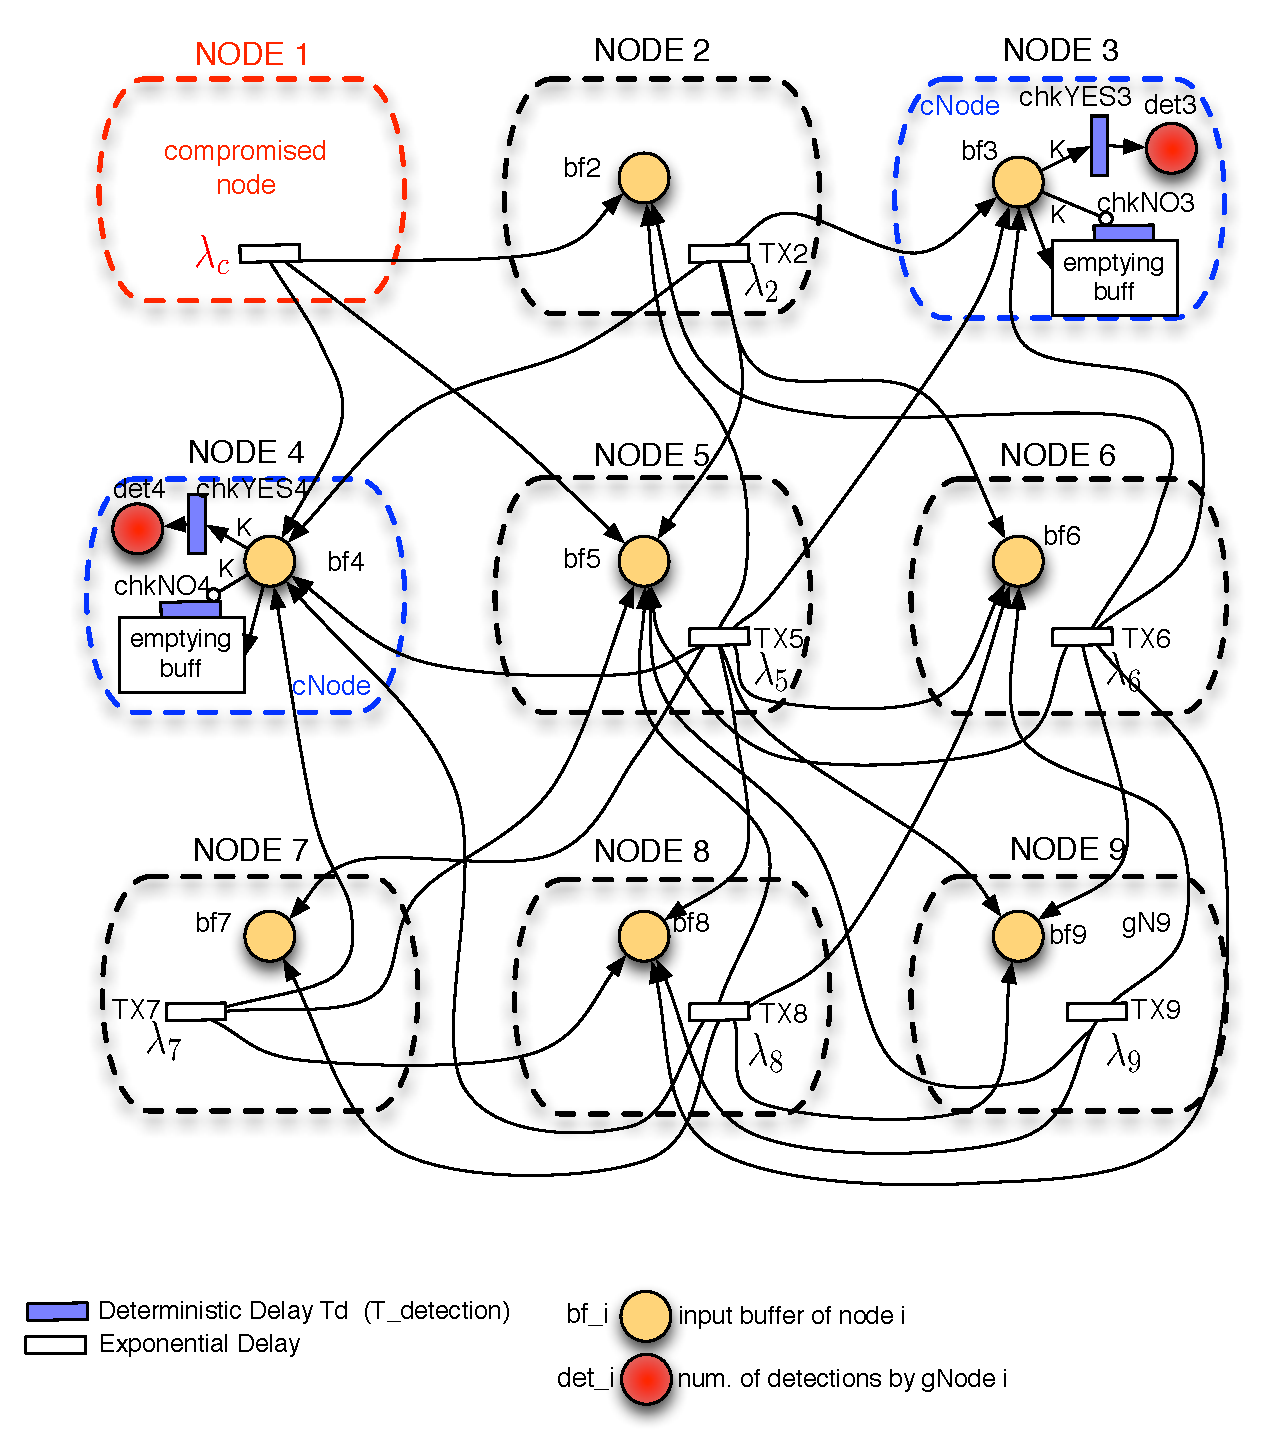
\includegraphics[width=\linewidth]{\chapterfig/PetriNet_DoS_9x9_fixedGnodes.pdf}
    \caption{Modèle RPSGE d'un cluster (topologie: grille $3\times3$) comprenant un nœud compromis et deux \cns statiques}\label{sa:fig:petricluster}
\end{figure}
Également dans l'optique de simplifier la représentation graphique, les transitions \textsf{e-on} et \textsf{e-end}, ainsi que la place \textsf{emptying buff}, ont été remplacées par une boîte blanche associée à la fonction de vidage de la place \textsf{In\_buff} des nœuds.

            \paragraph{\cns élus de façon dynamique}
L'élection dynamique des \cns vient compliquer un peu la modélisation de notre cluster.
Bien évidemment, tous les nœuds seront représentés selon le modèle ambivalent illustré par la figure~\ref{sa:fig:cnodegspn2}.
Mais il est aussi nécessaire de rajouter un module qui permettra l'élection des \cns pour chaque période.
Pour une meilleure clarté, le cluster sera représenté en deux temps.
Tout d'abord, la figure~\ref{sa:fig:petridyn} représente le cluster comme nous l'avons vu jusqu'ici, du point de vue du trafic.
\begin{figure}[ht]
    \centering
    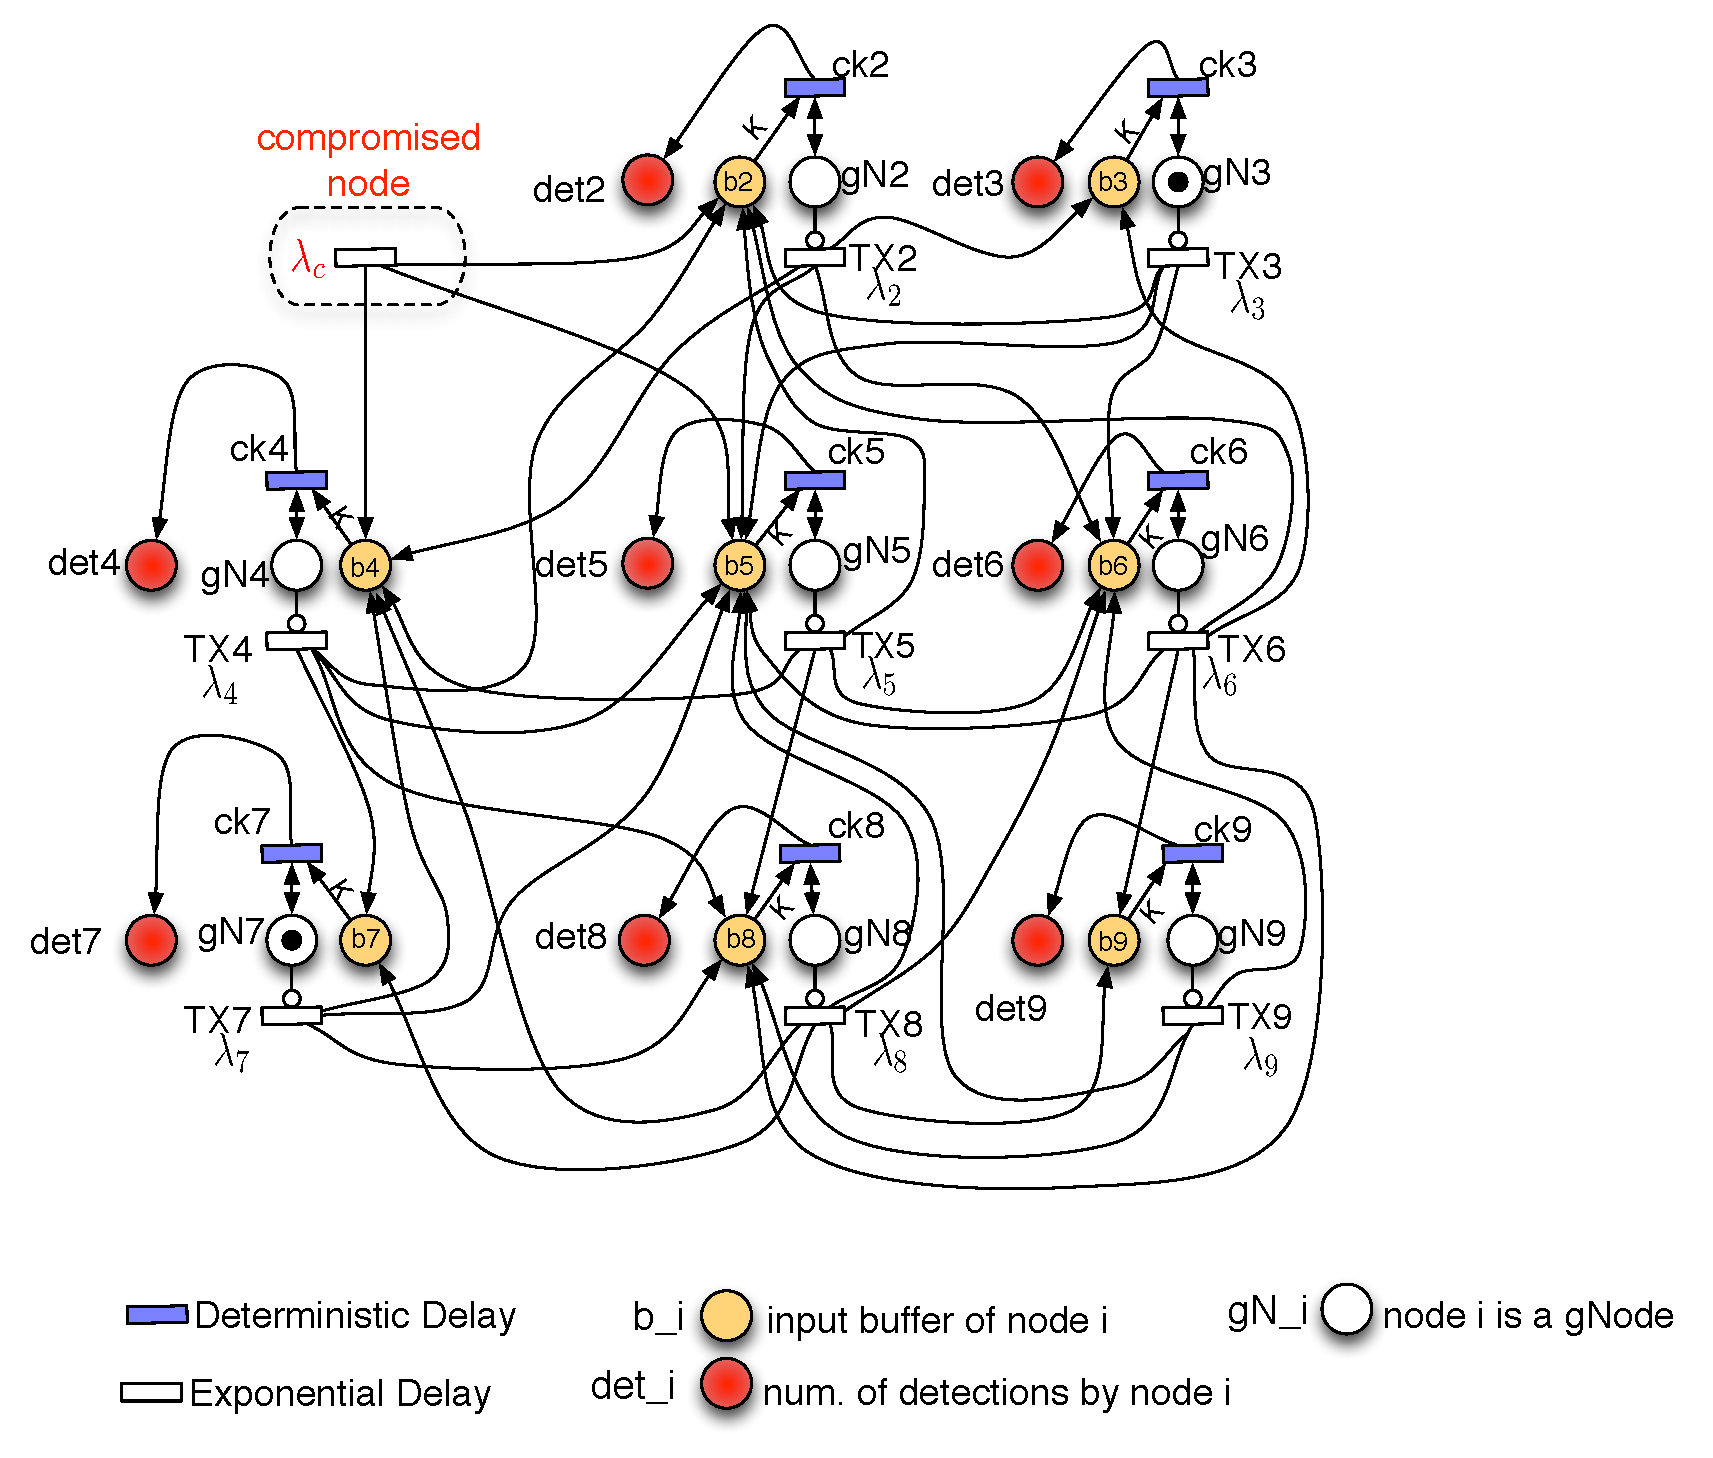
\includegraphics[width=\linewidth]{\chapterfig/PetriNet_DoS_9x9_noElection.pdf}
    \caption{Modèle RPSGE pour le trafic d'un cluster (topologie: grille $3\times3$) comprenant un nœud compromis et deux \cns élus de façon dynamique}\label{sa:fig:petridyn}
\end{figure}
Les huit nœuds non compromis peuvent endosser alternativement les rôles de capteur simple et de \cn (leur représentation a été simplifiée par rapport à la figure~\ref{sa:fig:cnodegspn2}).

\begin{figure}[ht]
    \centering
    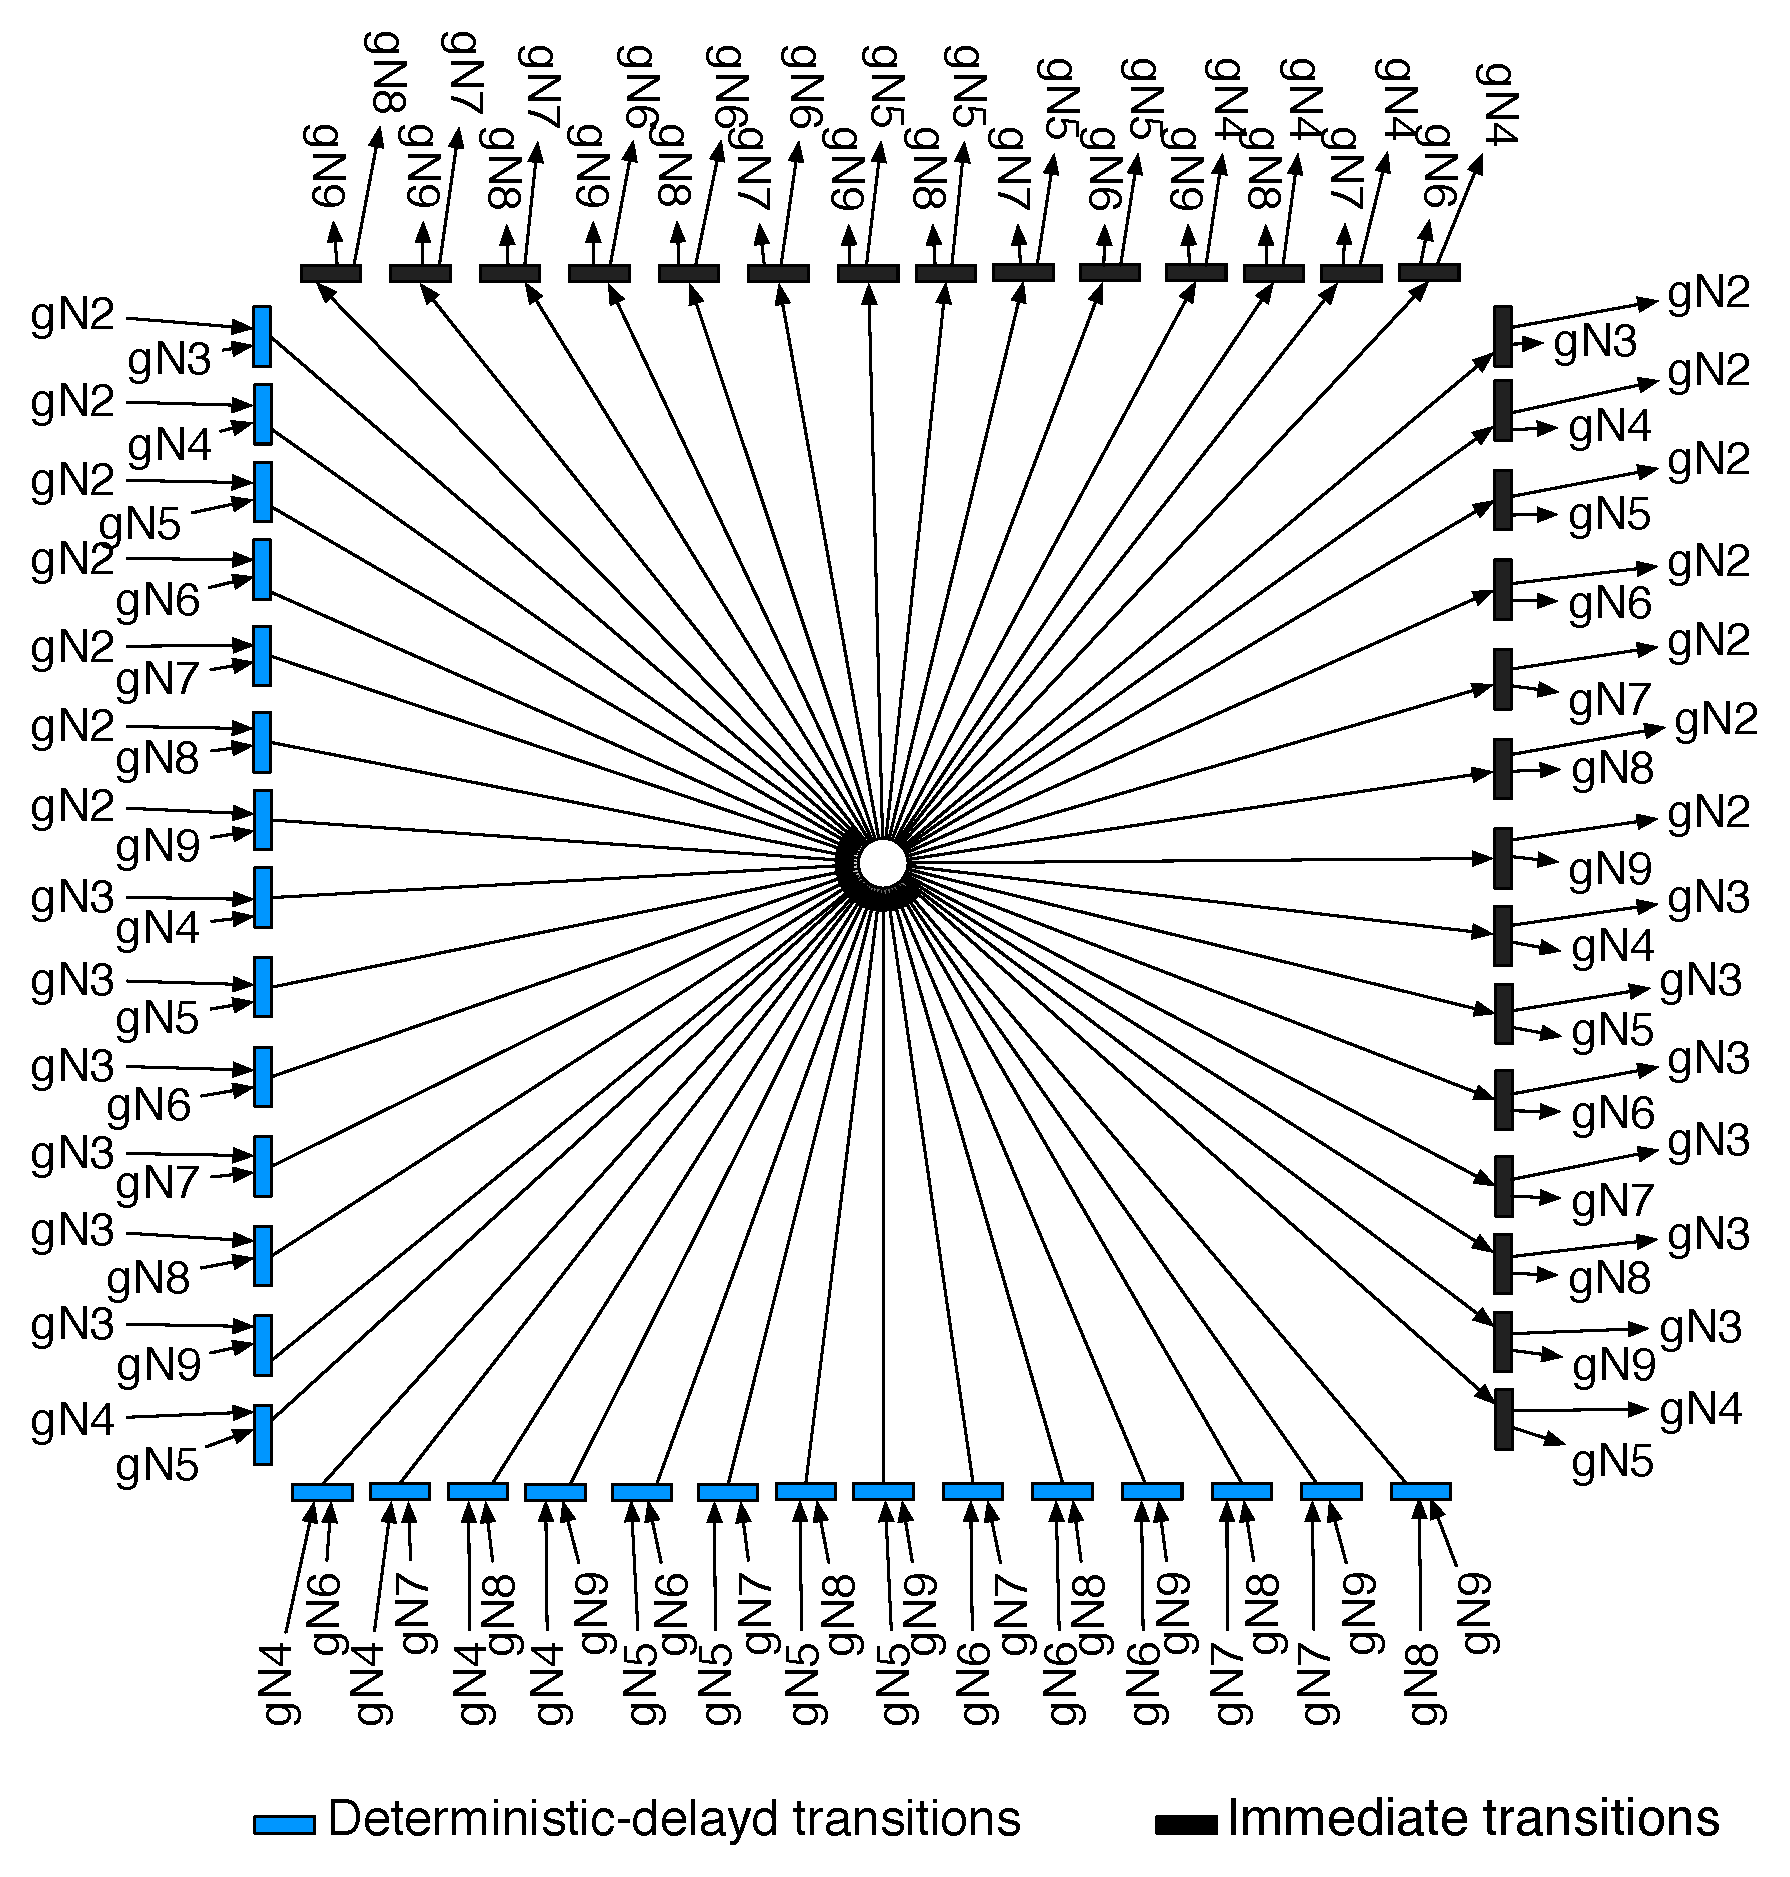
\includegraphics[width=\linewidth]{\chapterfig/PetriNet_DoS_9x9_gNodeElection.pdf}
    \caption{Modèle RPSGE pour l'élection dynamique de deux \cns parmi les nœuds du cluster}\label{sa:fig:petrielec}
\end{figure}
En considérant $n$ comme le nombre de résultats possibles à l'élection, le module représentant l'élection dynamique des \cns comprend:
\begin{itemize}
    \item une unique place centrale;
    \item $n$ transitions minutées, suivant une distribution déterministe, et mutuellement exclusives, menant à cette place (en bleu sur la figure~\ref{sa:fig:petrielec});
    \item $n$ transitions immédiates et mutuellement exclusives, franchissables depuis cette place (en noir sur la figure~\ref{sa:fig:petrielec}).
\end{itemize}
Dans notre cas, pour élire deux \cns au sein du cluster, et en supposant que le nœud compromis ne peut être élu, nous avons $n=\binom{8}{2}=28$~issues possible pour l'élection.
À la fin d'une période d'activité des \cns, une nouvelle élection est déclenchée.
La transition minutée correspondant aux \cns élus pour la période qui s'achève est déclenchée; les jetons présents dans les places \textsf{cNode} de ces \cns sont consommés, et produisent ainsi un jeton dans l'unique place centrale du module.
Chaque transition immédiate tente alors de produire un jeton.
Comme elles sont mutuellement exclusives, mais ont la même priorité et le même poids (voir \sssref{sa:subsubsec:presRPSGE}), un tirage aléatoire a lieu pour déterminer l'unique transition qui est franchie et produit ses jetons.
Ceux-ci sont envoyés dans les places \textsf{cNode} des nœuds élus pour la période qui débute, activant au passage leurs fonctionnalités de \cns.
%===============================================================================
    \subsection{Logique stochastique avec automates hybrides}

        \subsubsection{Présentation de la logique stochastique avec automates hybrides}
La logique stochastique avec automates hybrides (LSAH, ou bien \textit{Hybrid Automata Stochastic Logic}, \textit{HASL}) est un langage récent, qui introduit un framework regroupant des études de \textit{model checking} et d'évaluation des performances ainsi que de fiabilité sur des processus stochastiques à événements discrets (PSED) exprimés sous forme de réseaux de Petri sthochastiques généralisés (RPSG)~\cite{BDDHP11hasl}.
Plus concrètement, à partir d'un modèle RPSG, les mesures de performances sont exprimées à l'aide de formules LSAH avant que leur soit appliquées des fonctions de \textit{model checking} statique permettant de vérifier automatiquement ces formules.
%en place de vérifications, en termes d'études statistiques, de modèles stochastiques~\cite{BDDHP11hasl}.

Pour bien comprendre le fonctionnement de LSAH, voici quelques rappels sur le \textit{model checking}: il s'agit d'une procédure de vérification formelle utilisant:
\begin{itemize}
    \item un modèle $M$ à états discrets;
    \item une propriété formelle exprimée par une formule de logique temporelle $\phi$.
\end{itemize}
Un algorithme est alors utilisé pour déterminer automatiquement si $\phi$ vérifie $M$ (ce que l'on note $M\models\phi$).
Dans le cas d'un modèle stochastique, des probabilités sont associées aux formules.
Vérifier que $M\models\phi$ revient alors à déterminer la probabilité de la formule $\phi$ dans le contexte du modèle $M$.
LSAH étend ce concept dans le sens où l'évaluation d'une formule peut donner n'importe quel nombre réel, et représenter ainsi une probabilité aussi bien que toute autre mesure de performance.
À cette fin, LSAH fait appel à des automates linéaires hybrides (ALH).
Un ALH résulte, de manière résumée, de la généralisation des automates temporels dont les variables «~horloges~» sont remplacées par des variables de données réellement évaluées.
Basée sur ce modèle une formule LSAH comprend ainsi deux sous-éléments:
\begin{itemize}
    \item un ALH permettant la sélection des exécutions temporelles à retenir à partir du modèle RPSG considéré, cette sélection étant le fruit de la syncronisation entre une exécution générée par le modèle RPSG et l'ALH;
    \item une expression $Z$, représentant la mesure à évaluer, construite à l'aide des variables de l'ALH selon la syntaxe suivante:
    \[
        \begin{split}
            Z ::= & \ E(Y)\ |\ Z+Z\ |\ Z \times Z\\
            Y ::= & \ c\ |\ Y+Y\ |\ Y \times Y\ |\ Y/Y\ |\ \mbox{last}(y)\ |\ \mbox{min}(y)\\
                  & \ \  |\ \mbox{max}(y)\ |\ \mbox{int}(y)\ |\ \mbox{avg}(y)\\
            y ::= & \ c\ |\ x\ |\ y+y\ |\ y \times y\ |\ y/y
        \end{split}
    \]
    Cette expression peut être interprétée comme suit:
    \begin{itemize}
        \item $x$ est une variable de données de l'automate:
        \item $y$ est une expression arithmétique à partir de ces variables de données;
        \item $Y$ est une variable de chemin aléatoire, \cad une variable évaluée à l'aide d'un chemin de syncronisation, lui-même créé par la syncronisation entre une trajectoire du modèle RPSG et l'ALH;
        \item $\mbox{last}(y)$ est la dernière des valeurs endossées par l'expression $y$ le long d'un chemin syncronisé; $\mbox{min}(y)$ et $\mbox{max}(y)$ sont les valeurs optimales obtenues le long de ce chemin. $\mbox{int}(y)$ est l'intégrale d'$y$, et $\mbox{avg}(y)$ la moyenne des valeurs obtenues le long du chemin.
    \end{itemize}
\end{itemize}

Au final, LSAH fonctionne de la façon suivante:
\begin{enumerate}
    \item le système est exprimé sous la forme d'un modèle RPSG et d'une formule LSAH;
    \item LSAH génère de façon itérative les trajectoires à partir de l'espace d'états du modèle RPSG et les syncronise avec l'ALH;
    \item les trajectoires acceptées par l'ALH sont évaluées pour obtenir l'estimation de la mesure étudiée. Les trajectoires refusées sont abandonnées.
\end{enumerate}

        \subsubsection{Automate linéaire hybride et formule LSAH associés au modèle utilisé}
Nous présentons ici quelques exemples de formules LSAH, constitués des expressions LSAH et d'un automate hybride linéaire hybride (ALH) associé au modèle RPSGE présenté plus haut (en figure~\ref{sa:fig:petridyn}).
Ces exemples présentent une manière de mesurer des données sur un nœud du réseau de capteurs à partir de la version modélisée sous forme de réseaux de Petri, à fin d'étude, ou bien de comparaison de notre solution avec d'autres systèmes de détection des attaques de type «~déni de service~».
Ces exemples peuvent en outre être modélisés facilement avec l'outil de \textit{model checking} \textsf{COSMOS}~\cite{BDDHP11cosmos}.

On considère un nœud quelconque $i$ ($1\leq i\leq$~nombre de capteurs).
L'automate linéaire hybride que nous utilisons fait appel aux variables valuées suivantes:
\begin{itemize}
    \item $x_t$: temps global;
    \item $x_{d_i}$: nombre d'attaques détectées par le \cn $i$;
    \item $x_{\mathit{TX}_i}$: nombre de paquets envoyés par le nœud $i$;
    \item $x_{\mathit{bf}_i}$: nombre de paquets reçus et placés dans le tampon en entrée du nœud $i$.
\end{itemize}
L'automate linéaire hybride est présenté en figure~\ref{sa:fig:lha}.
\begin{figure}[ht]
    \centering
    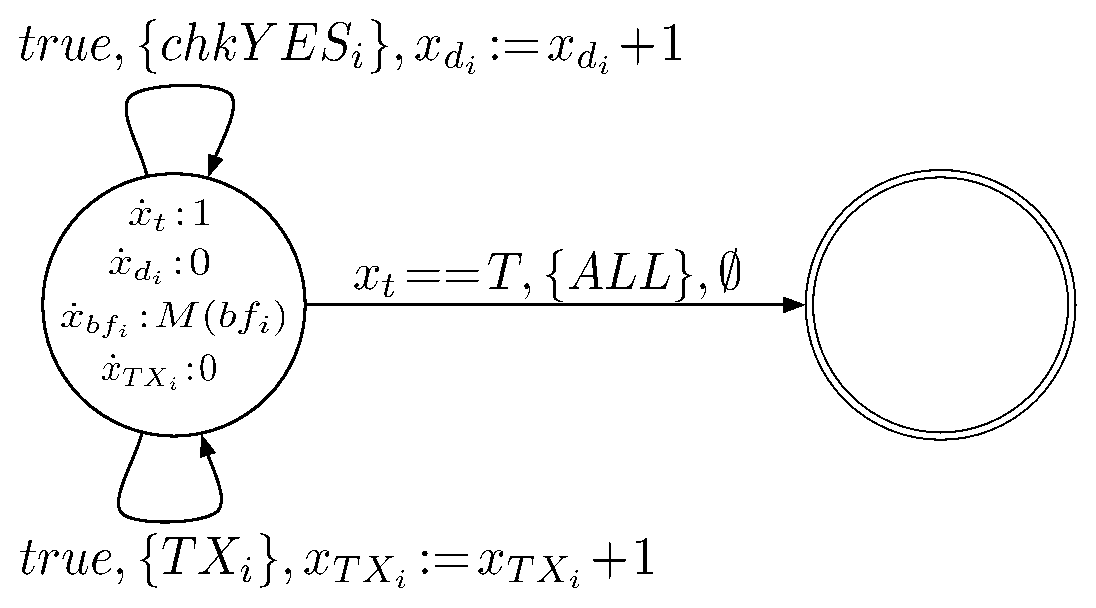
\includegraphics[width=.8\linewidth]{\chapterfig/LHA1.pdf}
    \caption{Automate linéaire hybride permettant d'effectuer des mesures sur le modèle RPSGE proposé}\label{sa:fig:lha}
\end{figure}
Cet automate comprend deux états, et fait références aux variables que nous venons de définir.
Ses transitions sont franchies lorsqu'un élément survient (par exemple: égalité de $x_t$ à $T$, ou franchissement d'une transition sur le modèle RPSGE); nous y reviendrons.
L'état de gauche, que l'on nommera $e_1$, contient le taux de variation (autrement dit, la dérivée première) de chacune des quatre variables décrites:
\begin{itemize}
    \item À chaque unité de temps passée, le temps global (la variable $x_t$) est incrémenté de $\dot{x}_t=1$;
    \item $x_{d_i}$ et $x_{\mathit{TX}_i}$ sont inchangées tant qu'aucune transition du modèle RPSGE n'est franchie.
        Leurs taux de variation $\dot{x}_{d_i}$ et $\dot{x}_{\mathit{TX}_i}$ sont nuls;
    \item $x_{\mathit{bf}_i}$ est incrémentée avec un taux proportionnel au nombre de jetons présents dans le tampon d'entrée de $i$ (lorsque $i$ joue le rôle de \cn).
        On notera ce taux $\dot{x}_{\mathit{bf}_i}$.
\end{itemize}
$e_1$ comporte également trois transitions, exprimées sous la forme suivante: $<$\textit{condition temporelle (sur x\_t)}$>, <$\textit{ensemble des transitions franchies sur le réseau de Petri pour déclencher l'évènement}$>, <$\textit{action associée sur les variables de l'automate}$>$.
Il s'agit des transitions suivantes:
\begin{itemize}
    \item la première transition qui boucle sur $e_1$: $e_1\xrightarrow{\mathit{true},\{\mathsf{chkYES_i}\},(x_{d_i}:=x_{d_i}+1)}{e_1}$.
        Elle correspond à l'évènement associé au passage de la transition \textsf{check\_YES} du nœud $i$ sur le modèle RPSGE du cluster (présenté en figure~\ref{sa:fig:petridyn}).
        Lorsque la transition est franchie sur le réseau de Petri, quelle que soit la valeur de l'«~horloge~» $x_t$ (condition $\mathit{true}$), la transition correspondante sur l'automate linéaire hybride est elle-aussi franchie\footnote{Attention: les transitions du réseau de Petri, représentées par des rectangles et reliées aux places par des arcs, ne doivent pas être confondues avec les transitions des automates, représentées par des arcs, et reliant les états.}.
        Comme la transition du réseau de Petri correspond à une nouvelle détection de trafic anormal par le nœud $i$, la transition de l'automate a pour effet de mettre à jour la valeur de $x_{d_i}$, en l'incrémentant de $1$;
    \item une deuxième transition qui boucle elle aussi sur $e_1$: $e_1\xrightarrow{\mathit{true},\{\mathsf{TX_i}\},(x_{\mathit{TX}_i}:=x_{\mathit{TX}_i}+1)}{e_1}$.
        Cette transition fonctionne de façon identique à la précédente, à la différence près que la transition du réseau de Petri concernée n'est plus \textsf{check\_YES} mais \textsf{TX}, et la variable de l'automate est $x_{\mathit{TX}_i}$: lorsque le nœud $i$ envoie un message (et que \textsf{TX} est franchie sur le modèle RPSGE), la variable $x_{\mathit{TX}_i}$ est incrémentée de $1$;
    \item une dernière transition qui mène de $e_1$ à $e_2$.
        Cette transition conduit à l'état final de l'automate, qui accepte et valide le chemin des transitions parcourues pour l'étudier à l'aide des formules LSAH: $e_1\xrightarrow{(x_t==T),\{\mathit{ALL}\},\emptyset}{e_2}$.
        La transition est autorisée lorsque $x_t$ vaut $T$, autrement dit: elle est déclenchée toutes les $T$ unités de temps.
        Elle accepte donc n'importe quel chemin dans l'automate, dont la durée est de $T$ unités de temps.
        Elle ne dépend pas d'une transition particulière du modèle RPSGE (puisqu'elle les acceptes toutes, $\{\mathit{ALL}\}$).
        Aucune action sur les variables n'est effectuée lorsque la transition est franchie.
\end{itemize}

Une fois un chemin validé par l'automate, il peut être analysé à l'aide de formule LSAH.
Voici quelques exemples de formules LSAH permettant d'obtenir plusieurs valeurs sur le cluster considéré à partir des variables définies plus haut pour l'automate:
\begin{itemize}
    \item $Z_1\equiv E(\mbox{last}(x_{d_i}))$: le nombre attendu d'attaques détectées par le \cn $i$ après $T$ unités de temps;
    \item $Z_2\equiv E(\mbox{last}(x_{d_i}+x_{d_{i'}}))$: la somme attendue des attaques détectées par les nœuds $i$ et $i'$ après $T$ unités de temps;
    \item $Z_3\equiv E(\mbox{last}(x_{\mathit{TX}_i}))$: le nombre attendu de paquets envoyés par le nœud $i$ après $T$ unités de temps;
    \item $Z_4\equiv E(\mbox{int}(x_{\mathit{bf}_i}))$: le cumul attendu du nombre de paquets reçus par le nœud $i$ après $T$ unités de temps.
\end{itemize}

%===============================================================================
    \subsection{Conclusion}

Ici se termine la section sur la modélisation.
Après avoir étudié les limites des processus markoviens, qui sont orientés vers la modélisation d'événements à distribution exponentielle, nous avons présenté deux autres évaluations formelles possibles pour notre solution.
L'une d'elles a fait intervenir une version étendue des réseaux de Petri, dédiée à la représentation de toutes sortes de distributions événementielles, et permet la visualisation de la solution sous l'aspect classique des réseaux de Petri.
La dernière est basée sur un langage récent, la logique stochastique avec automates hybrides, et permet l'évaluation formelle des performances de notre solution.
Toutes ont bien sûr pour objectif de modéliser notre solution afin d'en souligner les avantages et inconvénients, mais aussi de présenter aux lecteurs différents moyens existants d'employer les méthodes formelles en vue de modéliser des réseaux de capteurs, et ce de façon plus générale que dans le seul contexte de notre solution.

Évidemment, malgré tous ses attraits la modélisation ne peut se substituer à une évaluation numérique de la solution, comme nous allons le présenter, dans la section suivante, par le biais des résultats obtenus à l'aide d'une simulation.
